\documentclass[]{article}
\usepackage{xcolor}
\usepackage{listings}
\usepackage{showexpl}
\usepackage[bahasai]{babel}
\usepackage{graphicx}
\lstset{language=C++,
	% numbers=left,
	%	stepnumber=1,
	numberstyle=\ttfamily,
	basicstyle=\ttfamily,
	keywordstyle=\color{blue}\ttfamily,
	stringstyle=\color{red}\ttfamily,
	commentstyle=\color{gray}\ttfamily,
	morecomment=[l][\color{magenta}]{\#}
}


%opening
\title{Tugas 2: Implementasi Struktur Pada Array}
\author{Akhmad Thoriq Afif NRP 5024201028}

\begin{document}
\maketitle
\section{Listing Program}
Berikut ini merupakan kodingan dari tugas 2 Implementasi Struktur pada Array. Program ini dibuat dengan bahasa pemrograman C++.
\lstinputlisting[label={kodingan},caption={Implementasi Struktur pada Array}, language={C++}]{tugas.cpp}
\subsection*{OUTPUT PROGRAM:}
% add graphics
\begin{figure}[htp]
    \centering
    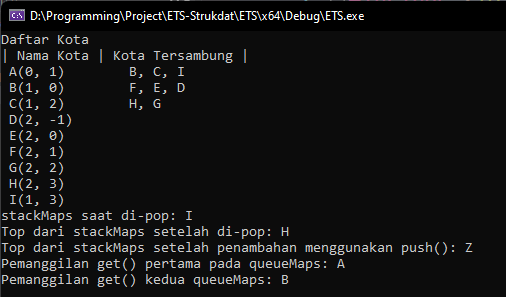
\includegraphics[width=8cm]{output.png}
    \caption{Output Program}
    \label{fig:galaxy}
\end{figure}
\pagebreak
\section{Penjelasan Program}
\subsection{Desain struktur data}
\par
Pada program ini terdapat struct Node yang merupakan representasi dari Kota. Dalam Node ini terdapat atribut nama kota, kota yang tersambung, dan koordinat kota. Selain Node, terdapat class Maps. Class Maps menyimpan Node-Node yang ada. Node tersebut disimpan kedalam sebuah array yang dapat ditentukan ukurannya.
\par
Di dalam struct Node terdapat array mConnected yang berfungsi untuk menyimpan kota yang tersambung ke kota tersebut. Objek yang disimpan dalam array ini berupa indeks kota yang tersambung. Hal ini dilakukan agar dapat mengakses kota yang tersambung lebih efisien ketimbang menggunakan nama kota atau ID tetap. Terutama ketika melakukan proses pathfinding. Pada proses pathfinding tiap-tiap kota yang tersambung akan diakses, jika menggunakan nama kota atau ID tetap maka akan terjadi pencarian kota secara berulang-ulang. Hal ini sangatlah tidak efisien. Maka dari itu digunakanlah indeks sebagai objek yang disimpan dalam array mConnected.
\subsection{Perubahan Kode}
Dibanding dengan program sebelumnya, pada program ini terdapat perbaikan pada fungsi remove() dan insert(). Sealin dilakukan perbaikan, terdapat penambahan pada fungsi addcity() dan conect(). Pada kedua fungsi tersebut ditambahkan return berupa this. Sehingga ketika dilakukan pemanggilan method tersebut, method tersebut dapat dipanggil kembali tanpa menyertakan objeknya.
\subsection{Fungsi untuk menambah kota}
\lstinputlisting[label={maxvalue},caption={Fungsi untuk menambah kota}, language={C++}, firstline=131, lastline=145]{tugas.cpp}
\par
Fungsi ini digunakan untuk menambahkan kota. Dibutuhkan 3 parameter yaitu nama kota dan koordinat kota. Langkah-langkah dalam menambah kota adalah sebagai berikut:
\begin{enumerate}
    \item Membuat object Node baru bernama newCity.
    \item Melakukan pengecekan ukuran Maps. Jika ukuran Maps masih cukup maka akan dilakukan penambahan kota.
    \item Pada akhir fungsi dilakukan pengembalian *this, sehingga fungsi ini dapat dipanggil kembali secara beruntun.
\end{enumerate}
\subsection{Fungsi untuk menghapus kota}
\lstinputlisting[label={hapusmaks},caption={Fungsi untuk menghapus kota}, language={C++}, firstline=148, lastline=162]{tugas.cpp}
\par
Fungsi ini digunakan untuk menghapus kota. Dibutuhkan 1 parameter yaitu nama kota. Langkah-langkah dalam menghapus kota adalah sebagai berikut:
\begin{enumerate}
    \item Melakukan pencarian index kota yang akan dihapus dengan menggunakan fungsi findCityByname.
    \item Memindahkan elemen sebelah kanan kota yang akan dihapus ke index kota yang akan dihapus. Proses ini dilakukan secara terus menerus sampai ujung array.
    \item Melakukan pengupdatean array mConnected yang terdapat pada setiap object Node. Pengupdatean ini akan dijabarkan pada penjelasan di bawah.
    \item Mengurangi ukuran Maps.
\end{enumerate}
\lstinputlisting[label={updatehapus},caption={Fungsi untuk mengupdate indeks kota}, language={C++}, firstline=37, lastline=58]{tugas.cpp}
\begin{enumerate}
    \item Melakukan transversal pada array mConnected.
    \item Melakukan pengecekan jika pada array mConnected terdapat index kota yang dihapus, maka akan dilakukan penghapusan elemen tersebut dari array mConnected.
    \item Melakukan pengurangan 1 nilai pada tiap-tiap index yang lebih besar dari index kota yang dihapus.
\end{enumerate}
\subsection{Fungsi untuk mencari kota}
\lstinputlisting[label={findcitybynama},caption={Fungsi untuk mencari kota}, language={C++}, firstline=174, lastline=184]{tugas.cpp}
\par
Fungsi ini digunakan untuk mencari kota. Dibutuhkan 1 parameter yaitu nama kota. Langkah-langkah dalam mencari kota adalah sebagai berikut:
\begin{enumerate}
    \item Melakukan transversal pada array maps. Jika nama kota yang dicari sama dengan nama kota pada array maka akan dikembalikan index kota.
    \item Jika tidak ada kota yang sama maka akan dikembalikan nilai -1.
\end{enumerate}
\subsection{Fungsi untuk menyisipkan kota}
\lstinputlisting[label={fungsiinsert},caption={Fungsi untuk menyisipkan kota}, language={C++}, firstline=109, lastline=129]{tugas.cpp}
\par
Fungsi ini digunakan untuk menyisipkan kota. Dibutuhkan 3 parameter yaitu nama kota, koordinat kota, dan indeks kota. Langkah-langkah dalam menyisipkan kota adalah sebagai berikut:
\begin{enumerate}
    \item Membuat object Node baru bernama newCity.
    \item Melakukan pengecekan ukuran Maps. Jika ukuran Maps masih cukup maka akan dilakukan penambahan kota.
    \item Melakukan pergeseran elemen n ke n+1, dimana n adalah elemen terakhir pada array mArray. Setelah dilakukan pergeseran n mundur ke n-1. Proses ini dilakukan berulang kali sampai n = index yang akan disisipkan.
    \item Melakukan pengisian elemen pada index n dengan newCity.
    \item Melakukan pengupdatean array mConnected yang terdapat pada setiap object Node.
    \item Menambahkan ukuran Maps dengan menambah mCurrSize dengan 1.
\end{enumerate}
\end{document}
